\title{Rank Effect and Individual Investors' Buying Decisions}
% \author{}
\date{\today}

% classes
\documentclass[12pt]{article}

\usepackage{todonotes}
\usepackage{amsmath,amssymb,amsfonts,amsthm}
\usepackage{graphicx}                           % Package to allow inclusion of graphics
% line spacing
\usepackage[onehalfspacing]{setspace}
\usepackage{booktabs}

\usepackage{rotating}



% define bibliography
\usepackage[backend=bibtex,style=authoryear,natbib=true,giveninits=true]{biblatex} % bibtex settings
\addbibresource{lit.bib}


\usepackage{geometry}
\geometry{a4paper,left=10mm,right=10mm, top=1cm, bottom=2cm}

\begin{document}
\maketitle

% \paragraph{Abstract}
% This can be used as a short abstract.

\section{Introduction}

\begin{figure}[h]
	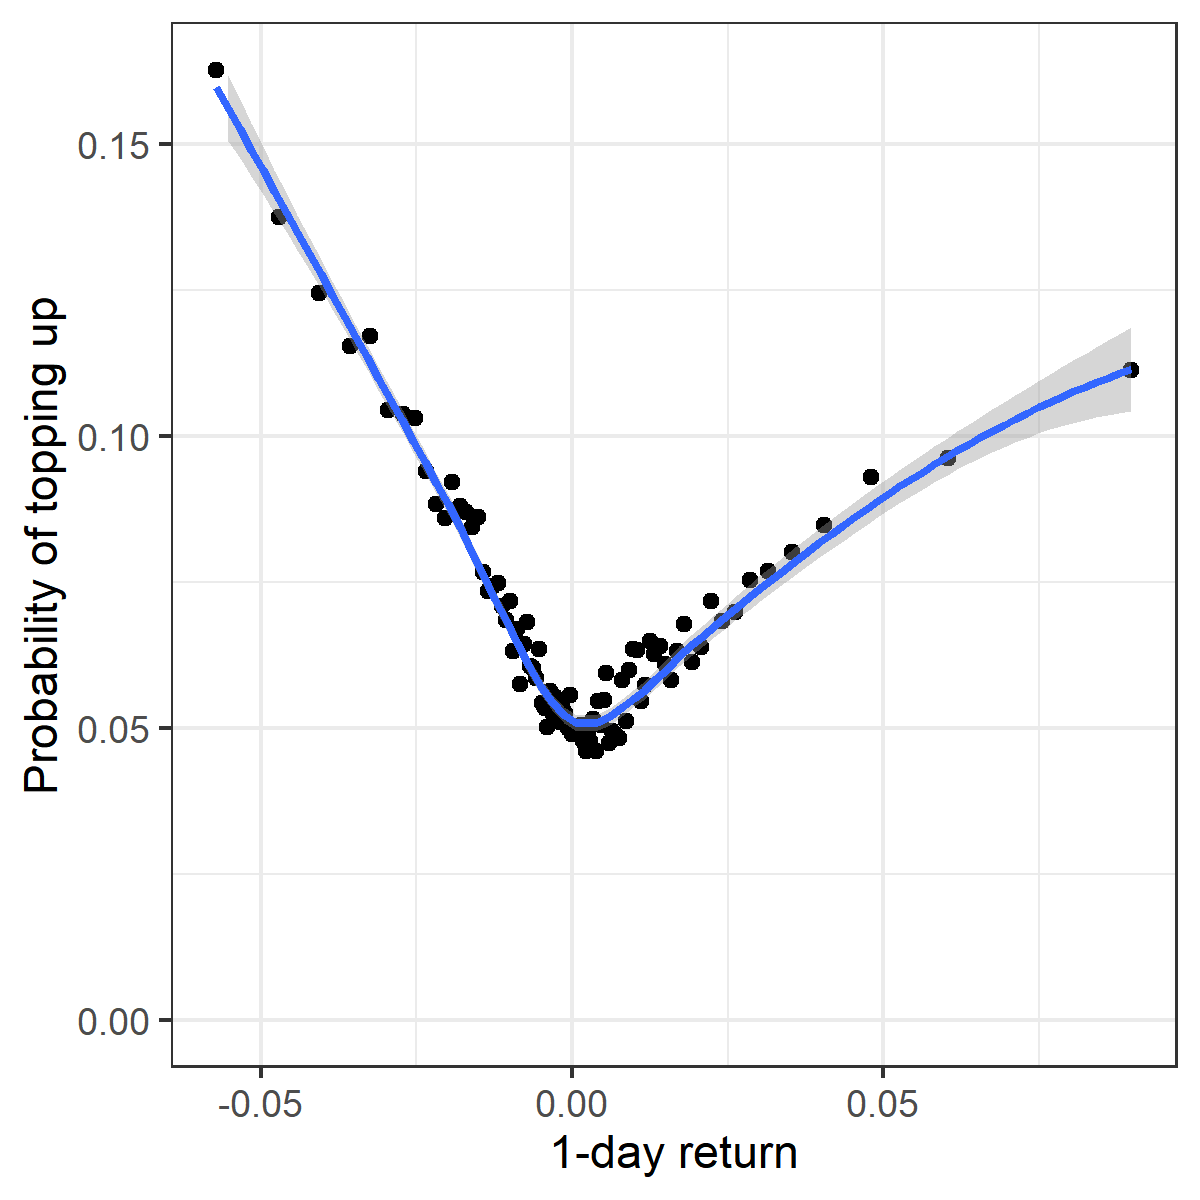
\includegraphics[scale=0.7]{figure_probtopup_1dayreturn}
	\centering
	\caption{Probability of topping up on each percentile of 1-day return}
\end{figure}

\begin{figure}[h]
	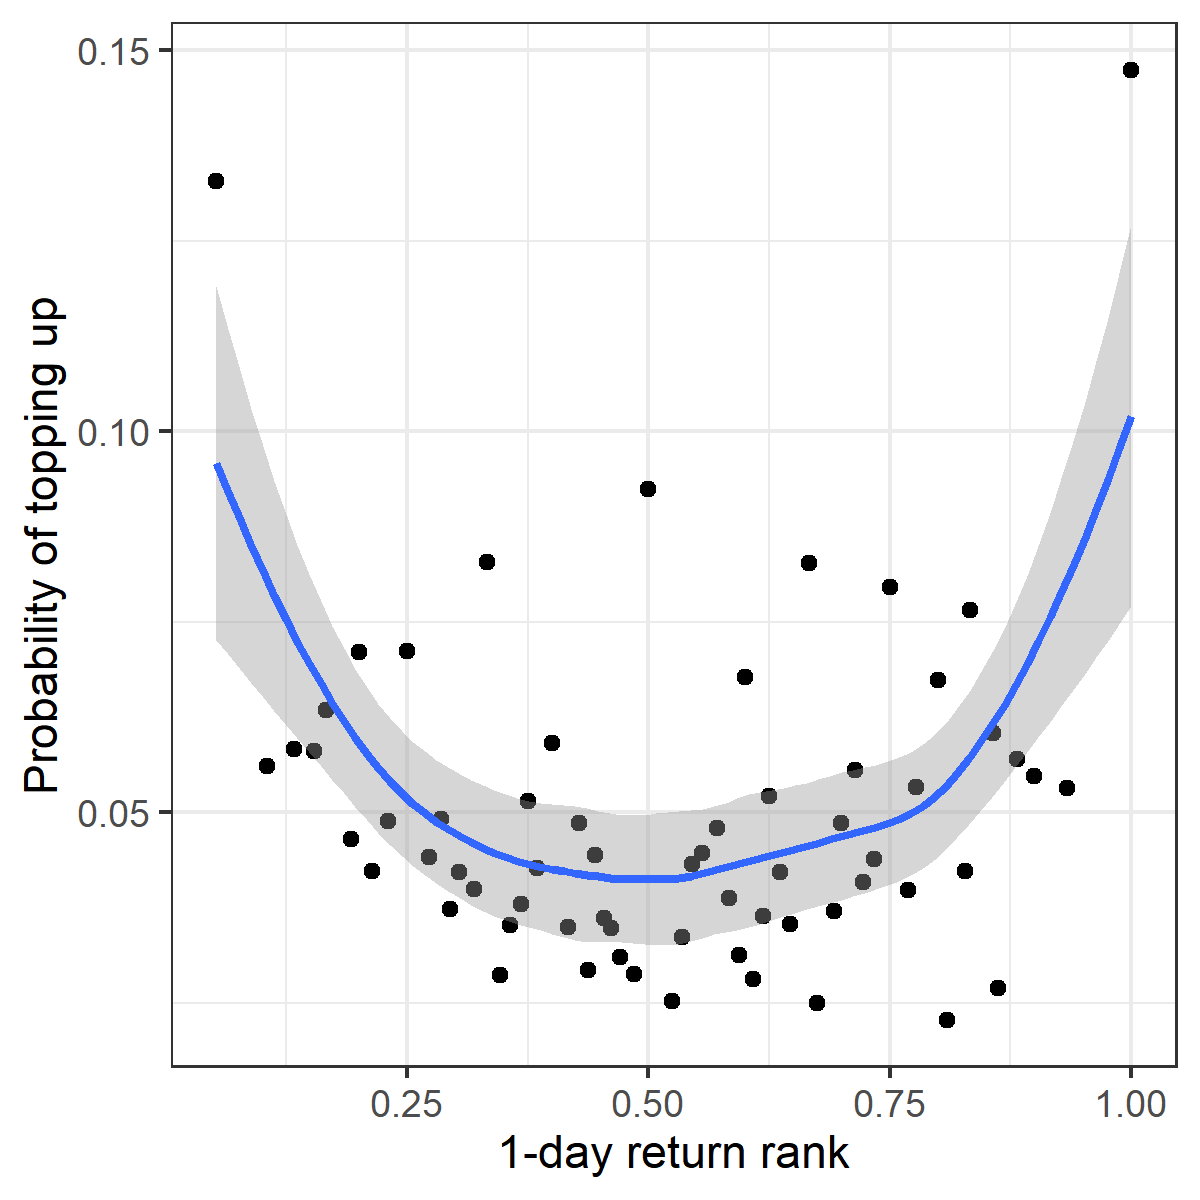
\includegraphics[scale=0.7]{figure_probtopup_1dayreturnrank}
	\centering
	\caption{Probability of topping up on 1-day return rank}
\end{figure}


\newpage

\section{Summary statistics}

 \subsection{Account level information}
 

% Table created by stargazer v.5.2.2 by Marek Hlavac, Harvard University. E-mail: hlavac at fas.harvard.edu
% Date and time: Mon, Mar 02, 2020 - 4:23:23 PM
\begin{table}[!htbp] \centering 
  \caption{Summary statistics at the account level: mean/median and (standard deviation)} 
  \label{} 
\begin{tabular}{@{\extracolsep{5pt}}lcccc} 
\\[-1.8ex]\hline 
\hline \\[-1.8ex] 
Variable & \multicolumn{1}{c}{N} & \multicolumn{1}{c}{Statistic}\\ 
\hline \\[-1.8ex] 
Age & 6,647 & 48.227/52.000 (14.947) \\ 
Top up rate & 6,654 & 0.122/0.096 (0.100) \\ 
\% Female &   & 17.9 \\ 
\hline \\[-1.8ex] 
\end{tabular} 
\end{table} 

 
 \subsection{Holding level information}


% Table created by stargazer v.5.2.2 by Marek Hlavac, Harvard University. E-mail: hlavac at fas.harvard.edu
% Date and time: Mon, Mar 02, 2020 - 3:19:20 PM
\begin{table}[!htbp] \centering 
  \caption{Summary statistics at the holding level} 
  \label{} 
\begin{tabular}{@{\extracolsep{5pt}}lcccccccc} 
\\[-1.8ex]\hline 
\hline \\[-1.8ex] 
Statistic & \multicolumn{1}{c}{N} & \multicolumn{1}{c}{Mean} & \multicolumn{1}{c}{St. Dev.} & \multicolumn{1}{c}{Min} & \multicolumn{1}{c}{Pctl(25)} & \multicolumn{1}{c}{Median} & \multicolumn{1}{c}{Pctl(75)} & \multicolumn{1}{c}{Max} \\ 
\hline \\[-1.8ex] 
1-day return & 1,111,928 & 0.0004 & 0.039 & $-$0.882 & $-$0.009 & 0.000 & 0.009 & 7.500 \\ 
rank 1-day return & 1,111,928 & 0.5333 & 0.255 & 0.000 & 0.346 & 0.500 & 0.714 & 1.000 \\ 
3-day return & 1,111,928 & 0.001 & 0.069 & $-$0.882 & $-$0.018 & 0.000 & 0.016 & 7.000 \\ 
rank 3-day return & 1,111,928 & 0.531 & 0.266 & 0.000 & 0.333 & 0.500 & 0.724 & 1.000 \\ 
1-week return & 1,111,928 & 0.002 & 0.090 & $-$0.999 & $-$0.024 & 0.000 & 0.022 & 8.062 \\ 
rank 1-week return & 1,111,928 & 0.529 & 0.275 & 0.000 & 0.300 & 0.500 & 0.700 & 1.000 \\ 
number of holdings & 1,111,928 & 16.021 & 15.644 & 3 & 7 & 11 & 20 & 128 \\ 
portfolio return & 1,111,928 & 0.012 & 0.146 & $-$0.988 & $-$0.053 & $-$0.00001 & 0.060 & 6.066 \\ 
\hline \\[-1.8ex] 
\end{tabular} 
\end{table} 


Daniel Stewart Securities increased from \pounds0.00200 to \pounds0.01700 (increased by $750\%$) from 30/March/2015 to 31/March/2015.

\newpage

\section{Top up decisions}

	

% Table created by stargazer v.5.2.2 by Marek Hlavac, Harvard University. E-mail: hlavac at fas.harvard.edu
% Date and time: Fri, Mar 06, 2020 - 5:32:45 PM
\begin{table}[!htbp] \centering 
  \caption{} 
  \label{} 
\begin{tabular}{@{\extracolsep{5pt}}lcccc} 
\\[-1.8ex]\hline 
\hline \\[-1.8ex] 
 & \multicolumn{4}{c}{\textit{Dependent variable:}} \\ 
\cline{2-5} 
\\[-1.8ex] & \multicolumn{4}{c}{Top Up} \\ 
\\[-1.8ex] & (1) & (2) & (3) & (4)\\ 
\hline \\[-1.8ex] 
 1-day rank & $-$0.274$^{***}$ & $-$0.071$^{***}$ & $-$0.079$^{***}$ &  \\ 
& (0.011) & (0.010) & (0.010) &  \\ 
& & & & \\
 1-day rank$^2$ & 0.286$^{***}$ & 0.091$^{***}$ & 0.085$^{***}$ &  \\ 
  & (0.010) & (0.009) & (0.009) &  \\ 
  & & & & \\ 
 1-day top rank &  &  &  & 0.029$^{***}$ \\ 
  &  &  &  & (0.003) \\ 
  & & & & \\ 
 1-day bottom rank &  &  &  & 0.022$^{***}$ \\ 
  &  &  &  & (0.003) \\ 
  & & & & \\ 
 Portfolio return &  &  & 0.031$^{***}$ & 0.029$^{***}$ \\ 
  &  &  & (0.008) & (0.007) \\ 
  & & & & \\ 
 Return since purchase &  &  & $-$0.059$^{***}$ & $-$0.059$^{***}$ \\ 
  &  &  & (0.013) & (0.013) \\ 
  & & & & \\ 
 Return since purchase rank &  &  & 0.038$^{***}$ & 0.039$^{***}$ \\ 
  &  &  & (0.005) & (0.004) \\ 
  & & & & \\ 
  $\sqrt{Holding\:days}$&  &  & $-$0.007$^{***}$ & $-$0.007$^{***}$ \\ 
  &  &  & (0.0002) & (0.0002) \\ 
  & & & & \\ 
Return since purchase$\times$ &  &  & 0.002$^{***}$ & 0.002$^{***}$ \\ 
 $\sqrt{Holding\:days}$&  &  & (0.001) & (0.001) \\ 
  & & & & \\ 
 
 Constant & 0.116$^{***}$ &  &  &  \\ 
  & (0.003) &  &  &  \\ 
  & & & & \\ 
\hline \\[-1.8ex] 
Account FE & No & Yes & Yes & Yes \\ 
Stock$\times$Date FE & No & Yes & Yes & Yes \\ 
Return decile FE & No & Yes & Yes & Yes \\ 
Observations & 1,111,928 & 1,111,928 & 1,111,928 & 1,111,928 \\ 
Adjusted R$^{2}$ & 0.009 & $-$0.004 & 0.019 & 0.019 \\ 
\hline 
\hline \\[-1.8ex] 
\textit{Note:}  & \multicolumn{4}{r}{$^{*}$p$<$0.05; $^{**}$p$<$0.01; $^{***}$p$<$0.005} \\ 
\end{tabular} 
\end{table} 



% Table created by stargazer v.5.2.2 by Marek Hlavac, Harvard University. E-mail: hlavac at fas.harvard.edu
% Date and time: Mon, Mar 02, 2020 - 6:40:29 PM
\begin{table}[!htbp] \centering 
	\caption{} 
	\label{} 
	\begin{tabular}{@{\extracolsep{5pt}}lcccc} 
		\\[-1.8ex]\hline 
		\hline \\[-1.8ex] 
		& \multicolumn{4}{c}{\textit{Dependent variable:}} \\ 
		\cline{2-5} 
		\\[-1.8ex] & \multicolumn{4}{c}{Top Up} \\ 
		\\[-1.8ex] & \multicolumn{2}{c}{N=3}& \multicolumn{2}{c}{N=5} \\
		\cmidrule(lr){2-3}
		\cmidrule(lr){4-5}
		\\[-1.8ex] & (1) & (2) & (1) & (2)\\ 
		\hline \\[-1.8ex] 
		
		
 N-day rank & $-$0.059$^{***}$ &  & $-$0.059$^{***}$ &  \\ 
& (0.010) &  & (0.010) &  \\ 
& & & & \\ 
N-day rank$^2$ & 0.068$^{***}$ &  & 0.067$^{***}$ &  \\ 
& (0.009) &  & (0.008) &  \\ 
& & & & \\ 
N-day top rank &  & 0.026$^{***}$ &  & 0.025$^{***}$ \\ 
&  & (0.003) &  & (0.003) \\ 
& & & & \\ 
N-day bottom rank &  & 0.019$^{***}$ &  & 0.021$^{***}$ \\ 
&  & (0.003) &  & (0.003) \\ 
& & & & \\ 	
\hline \\[-1.8ex] 	
Controls & Yes & Yes & Yes & Yes \\ 
Account FE & Yes & Yes & Yes & Yes \\ 
Stock$\times$Date FE & Yes & Yes & Yes & Yes \\ 
Return decile FE & Yes & Yes & Yes & Yes \\ 
Observations & 1,111,928 & 1,111,928 & 1,111,928 & 1,111,928 \\ 
R$^{2}$ & 0.419 & 0.419 & 0.419 & 0.419 \\ 
\hline 
\hline \\[-1.8ex] 
\textit{Note:}  & \multicolumn{4}{r}{$^{*}$p$<$0.05; $^{**}$p$<$0.01; $^{***}$p$<$0.005} \\ 
\end{tabular} 
\end{table} 


\begin{sidewaystable}
	\centering
	\small
	\caption{Subsample analysis: break by median house price}
	\begin{tabular}{ll}

% Table created by stargazer v.5.2.2 by Marek Hlavac, Harvard University. E-mail: hlavac at fas.harvard.edu




\begin{tabular}{@{\extracolsep{2pt}}lcccccccccccc} 
		\\[-1.8ex]\hline 
\hline \\[-1.8ex] 
& \multicolumn{12}{c}{\textit{Dependent variable:}} \\ 
\cline{2-13} 
\\[-1.8ex] & \multicolumn{12}{c}{Top Up} \\ 
\\[-1.8ex] & \multicolumn{6}{c}{high house price group}& \multicolumn{6}{c}{low house price group} \\
\cmidrule(lr){2-7}
\cmidrule(lr){8-13}
\\[-1.8ex] & \multicolumn{2}{c}{N=1}& \multicolumn{2}{c}{N=3}& \multicolumn{2}{c}{N=5}&\multicolumn{2}{c}{N=1}& \multicolumn{2}{c}{N=3}& \multicolumn{2}{c}{N=5} \\
\cmidrule(lr){2-3}
\cmidrule(lr){4-5}
\cmidrule(lr){6-7}
\cmidrule(lr){8-9}
\cmidrule(lr){10-11}
\cmidrule(lr){12-13}
\\[-1.8ex] & (1) & (2) & (1) & (2)& (1) & (2) & (1) & (2)& (1) & (2) & (1) & (2)\\ 
\hline \\[-1.8ex] 
N-day rank & $-$0.090$^{***}$ &  & $-$0.071$^{***}$ &  & $-$0.063$^{***}$ &  & $-$0.086$^{***}$ &  & $-$0.065$^{***}$ &  & $-$0.070$^{***}$ &  \\ 
& (0.018) &  & (0.017) &  & (0.017) &  & (0.019) &  & (0.018) &  & (0.017) &  \\ 
& & & & & & & & & & & & \\ 
N-day rank$^2$ & 0.090$^{***}$ &  & 0.074$^{***}$ &  & 0.067$^{***}$ &  & 0.097$^{***}$ &  & 0.079$^{***}$ &  & 0.079$^{***}$ &  \\ 
& (0.015) &  & (0.015) &  & (0.014) &  & (0.016) &  & (0.015) &  & (0.015) &  \\ 
& & & & & & & & & & & & \\ 
N-day top rank &  & 0.028$^{***}$ &  & 0.024$^{***}$ &  & 0.022$^{***}$ &  & 0.032$^{***}$ &  & 0.031$^{***}$ &  & 0.029$^{***}$ \\ 
&  & (0.004) &  & (0.005) &  & (0.004) &  & (0.005) &  & (0.005) &  & (0.004) \\ 
& & & & & & & & & & & & \\ 
N-day bottom rank &  & 0.027$^{***}$ &  & 0.023$^{***}$ &  & 0.025$^{***}$ &  & 0.021$^{***}$ &  & 0.019$^{***}$ &  & 0.020$^{***}$ \\ 
&  & (0.006) &  & (0.006) &  & (0.005) &  & (0.007) &  & (0.006) &  & (0.006) \\ 
& & & & & & & & & & & & \\ 

\hline \\[-1.8ex] 
Controls & Yes & Yes & Yes & Yes & Yes & Yes  & Yes & Yes & Yes & Yes & Yes & Yes \\ 
Account FE & Yes & Yes & Yes & Yes & Yes & Yes  & Yes & Yes & Yes & Yes & Yes & Yes \\ 
Stock*Date FE & Yes & Yes & Yes & Yes & Yes & Yes  & Yes & Yes & Yes & Yes & Yes & Yes  \\ 
Return decile FE & Yes & Yes & Yes & Yes & Yes & Yes  & Yes & Yes & Yes & Yes & Yes & Yes\\ 
Observations & 544,467 & 544,467 & 544,467 & 544,467 & 544,467 & 544,467 & 477,412 & 477,412 & 477,412 & 477,412 & 477,412 & 477,412 \\ 

Adjusted R$^{2}$ & $-$0.017 & $-$0.016 & $-$0.017 & $-$0.017 & $-$0.017 & $-$0.017 & 0.002 & 0.002 & 0.002 & 0.002 & 0.002 & 0.002 \\ 

\hline 
\hline \\[-1.8ex] 
\textit{Note:}  & \multicolumn{12}{r}{$^{*}$p$<$0.05; $^{**}$p$<$0.01; $^{***}$p$<$0.005} \\ 
\end{tabular} 


	\end{tabular}
\end{sidewaystable}
	




\newpage

\section{Extention: first buy}


% Table created by stargazer v.5.2.2 by Marek Hlavac, Harvard University. E-mail: hlavac at fas.harvard.edu
% Date and time: Mon, Mar 02, 2020 - 7:23:22 PM
\begin{table}[!htbp] \centering 
  \caption{Result with 30-day assumption} 
  \label{} 
\begin{tabular}{@{\extracolsep{5pt}}lcccccc} 
\\[-1.8ex]\hline 
\hline \\[-1.8ex] 
 & \multicolumn{6}{c}{\textit{Dependent variable:}} \\ 
\cline{2-7} 
\\[-1.8ex] & \multicolumn{6}{c}{First Buy} \\ 
\\[-1.8ex] & \multicolumn{2}{c}{N=1}& \multicolumn{2}{c}{N=3}& \multicolumn{2}{c}{N=5} \\
\cmidrule(lr){2-3}
\cmidrule(lr){4-5}
\cmidrule(lr){6-7}
\\[-1.8ex] & (1) & (2) & (1) & (2) & (1) & (2)\\ 
\hline \\[-1.8ex]
  N-day rank & $-$0.190$^{***}$ &  & $-$0.154$^{***}$ &  & $-$0.114$^{***}$ &  \\ 
  & (0.036) &  & (0.034) &  & (0.034) &  \\ 
  & & & & & & \\  
  N-day rank$^2$  & 0.218$^{***}$ &  & 0.190$^{***}$ &  & 0.159$^{***}$ &  \\ 
  & (0.032) &  & (0.031) &  & (0.031) &  \\ 
  & & & & & & \\ 
  N-day top rank &  & 0.066$^{***}$ &  & 0.060$^{***}$ &  & 0.054$^{***}$ \\ 
  &  & (0.010) &  & (0.009) &  & (0.034) \\ 
  & & & & & & \\ 
  N-day bottom rank &  & 0.055$^{***}$ &  & 0.037$^{***}$ &  & 0.026$^{**}$ \\ 
  &  & (0.010) &  & (0.010) &  & (0.010) \\ 
  & & & & & & \\ 
 portfolio\_return & 0.049 & 0.030 & 0.053 & 0.031 & 0.056 & 0.032 \\ 
  & (0.039) & (0.037) & (0.039) & (0.037) & (0.039) & (0.038) \\ 
  & & & & & & \\ 
\hline \\[-1.8ex] 
Account FE & Yes & Yes & Yes & Yes & Yes & Yes \\ 
Stock*Date FE & Yes & Yes & Yes & Yes & Yes & Yes \\ 
Return decile FE & Yes & Yes & Yes & Yes & Yes & Yes \\ 
Observations & 261,708 & 261,708 & 261,708 & 261,708 & 261,708 & 261,708 \\ 
Adjusted R$^{2}$ & 0.320 & 0.320 & 0.320 & 0.320 & 0.320 & 0.320 \\ 
\hline 
\hline \\[-1.8ex] 
\textit{Note:}  & \multicolumn{6}{r}{$^{*}$p$<$0.05; $^{**}$p$<$0.01; $^{***}$p$<$0.005} \\ 
\end{tabular} 
\end{table} 



% Table created by stargazer v.5.2.2 by Marek Hlavac, Harvard University. E-mail: hlavac at fas.harvard.edu
% Date and time: Mon, Mar 02, 2020 - 7:23:22 PM
\begin{table}[!htbp] \centering 
  \caption{Result with 60-day assumption} 
  \label{} 
\begin{tabular}{@{\extracolsep{5pt}}lcccccc} 
\\[-1.8ex]\hline 
\hline \\[-1.8ex] 
 & \multicolumn{6}{c}{\textit{Dependent variable:}} \\ 
\cline{2-7} 
\\[-1.8ex] & \multicolumn{6}{c}{First Buy} \\ 
\\[-1.8ex] & \multicolumn{2}{c}{N=1}& \multicolumn{2}{c}{N=3}& \multicolumn{2}{c}{N=5} \\
\cmidrule(lr){2-3}
\cmidrule(lr){4-5}
\cmidrule(lr){6-7}
\\[-1.8ex] & (1) & (2) & (1) & (2) & (1) & (2)\\ 
\hline \\[-1.8ex]
  N-day rank & $-$0.188$^{***}$ &  & $-$0.142$^{***}$ &  & $-$0.111$^{***}$ &  \\ 
  & (0.026) &  & (0.025) &  & (0.023) &  \\ 
  & & & & & & \\  
  N-day rank$^2$  & 0.203$^{***}$ &  & 0.171$^{***}$ &  & 0.143$^{***}$ &  \\ 
  & (0.024) &  & (0.022) &  & (0.021) &  \\ 
  & & & & & & \\ 
  N-day top rank &  & 0.058$^{***}$ &  & 0.055$^{***}$ &  & 0.048$^{***}$ \\ 
  &  & (0.007) &  & (0.006) &  & (0.006) \\ 
  & & & & & & \\ 
  N-day bottom rank &  & 0.058$^{***}$ &  & 0.037$^{***}$ &  & 0.028$^{***}$ \\ 
  &  & (0.008) &  & (0.007) &  & (0.007) \\ 
  & & & & & & \\ 
 portfolio\_return & 0.024 & 0.011 & 0.033 & 0.016 & 0.033 & 0.015 \\ 
  & (0.025) & (0.024) & (0.025) & (0.024) & (0.025) & (0.024) \\ 
  & & & & & & \\ 
\hline \\[-1.8ex] 
Account FE & Yes & Yes & Yes & Yes & Yes & Yes \\ 
Stock*Date FE & Yes & Yes & Yes & Yes & Yes & Yes \\ 
Return decile FE & Yes & Yes & Yes & Yes & Yes & Yes \\ 
Observations & 373,594 & 373,594 & 373,594 & 373,594 & 373,594 & 373,594 \\ 
Adjusted R$^{2}$ & 0.299 & 0.300 & 0.299 & 0.299 & 0.299 &  0.299 \\ 
\hline 
\hline \\[-1.8ex] 
\textit{Note:}  & \multicolumn{6}{r}{$^{*}$p$<$0.05; $^{**}$p$<$0.01; $^{***}$p$<$0.005} \\ 
\end{tabular} 
\end{table} 



% Table created by stargazer v.5.2.2 by Marek Hlavac, Harvard University. E-mail: hlavac at fas.harvard.edu
% Date and time: Mon, Mar 02, 2020 - 7:23:22 PM
\begin{table}[!htbp] \centering 
  \caption{Result with 90-day assumption} 
  \label{} 
\begin{tabular}{@{\extracolsep{5pt}}lcccccc} 
\\[-1.8ex]\hline 
\hline \\[-1.8ex] 
 & \multicolumn{6}{c}{\textit{Dependent variable:}} \\ 
\cline{2-7} 
\\[-1.8ex] & \multicolumn{6}{c}{First Buy} \\ 
\\[-1.8ex] & \multicolumn{2}{c}{N=1}& \multicolumn{2}{c}{N=3}& \multicolumn{2}{c}{N=5} \\
\cmidrule(lr){2-3}
\cmidrule(lr){4-5}
\cmidrule(lr){6-7}
\\[-1.8ex] & (1) & (2) & (1) & (2) & (1) & (2)\\ 
\hline \\[-1.8ex]
  N-day rank & $-$0.178$^{***}$ &  & $-$0.141$^{***}$ &  & $-$0.107$^{***}$ &  \\ 
  & (0.021) &  & (0.020) &  & (0.019) &  \\ 
  & & & & & & \\  
  N-day rank$^2$  & 0.189$^{***}$ &  & 0.165$^{***}$ &  & 0.135$^{***}$ &  \\ 
  & (0.019) &  & (0.018) &  & (0.017) &  \\ 
  & & & & & & \\ 
  N-day top rank &  & 0.052$^{***}$ &  & 0.053$^{***}$ &  & 0.045$^{***}$ \\ 
  &  & (0.006) &  & (0.005) &  & (0.005) \\ 
  & & & & & & \\ 
  N-day bottom rank &  & 0.057$^{***}$ &  & 0.037$^{***}$ &  & 0.028$^{***}$ \\ 
  &  & (0.006) &  & (0.006) &  & (0.006) \\ 
  & & & & & & \\ 
 portfolio\_return & 0.019 & 0.007 & 0.027 & 0.013 & 0.027 & 0.011 \\ 
  & (0.019) & (0.018) & (0.019) & (0.018) & (0.019) & (0.018) \\ 
  & & & & & & \\ 
\hline \\[-1.8ex] 
Account FE & Yes & Yes & Yes & Yes & Yes & Yes \\ 
Stock*Date FE & Yes & Yes & Yes & Yes & Yes & Yes \\ 
Return decile FE & Yes & Yes & Yes & Yes & Yes & Yes \\ 
Observations & 467,781 & 467,781 & 467,781 & 467,781 & 467,781 & 467,781 \\ 
Adjusted R$^{2}$ & 0.280 & 0.280 & 0.280 & 0.280 & 0.279 &  0.280 \\ 
\hline 
\hline \\[-1.8ex] 
\textit{Note:}  & \multicolumn{6}{r}{$^{*}$p$<$0.05; $^{**}$p$<$0.01; $^{***}$p$<$0.005} \\ 
\end{tabular} 
\end{table} 


\newpage

\section{Conclusion}
Here is a conclusion \citep{hartzmark2015worst}.

% makes automatic header
\printbibliography


\end{document}

  